\documentclass{../source/Experiment}

\major{信息工程}
\name{姚桂涛}
\title{叠加定理实验研究}
\stuid{3190105597}
\college{信息与电子工程学院}
\date{\today}
\lab{东4-216}
\course{电子电路设计实验}
\instructor{李锡华、施红军、叶险峰}
\grades{}
\expname{叠加定理实验研究}
\exptype{研究实验}
\partner{杜秉哲}

\begin{document}
    \makecover
    \makeheader

    \section{实验目的}
        \begin{enumerate}
            \item 实验研究叠加定理的正确性;
            \item 加深叠加定理适用范围的认识。 
        \end{enumerate}
    \section{实验任务和要求}
        \begin{enumerate}
            \item 按电路图连接好电路。
            \item 在节点 F,E 之间接入电压源 $U_1$,$U_2$处不接电源,将节点 B,C短接,测量各点电压与各支路电流。
            \item $U_1$处不接电源,将节点 F,E 之间短路,在节点 B,C 之间接入电压源 $U_2$,再次测量各点电压与各支路电流。
            \item 同时接上电压源 $U_1$和$U_2$,重复上述测量。
            \item 再用二极管$D1$代替$R5$,重复实验。 
        \end{enumerate}
    \section{实验方案设计与实验参数计算}
        \subsection{完整的实验电路}
            \begin{figure}[htbp]
                \begin{center}
                    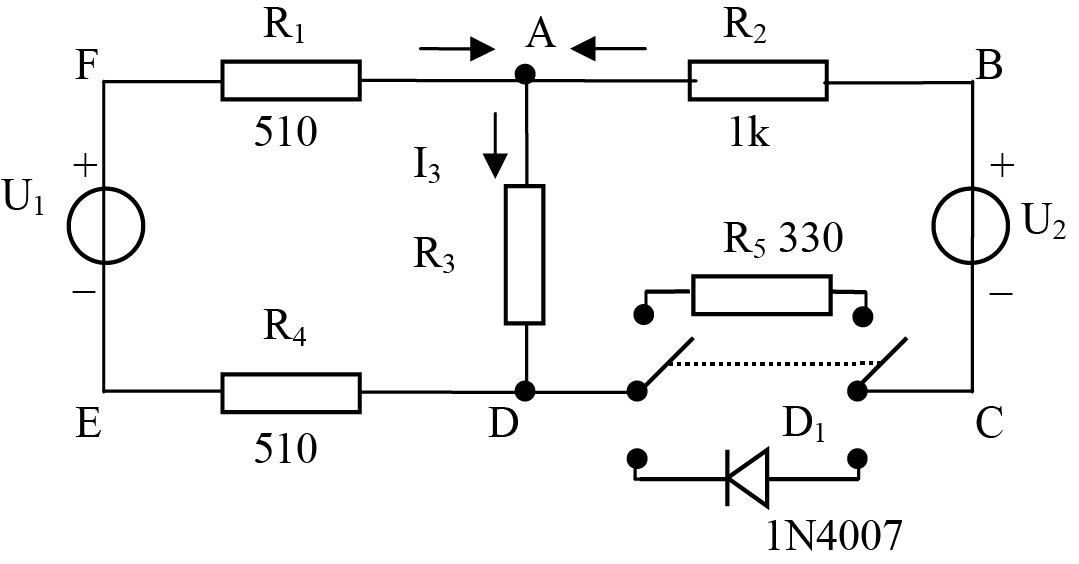
\includegraphics{pic/pic2.png}
                    \caption{验证叠加定理的实验电路}
                \end{center}
            \end{figure}
        \subsection{实验方案总体设计}
            \begin{enumerate}
                \item 接入电阻$R_5$。
                \item 分别让$U_1$单独作用,$U_2$单独作用,$U_1$、$U_2$共同作用时(另外一个电压源不作用时,将其短接),测量各点电压与支路电流。验证叠加定理在线性电路中是否成立。
                \item 将$R_5$替换为二极管$D_1$,重复上述测量,验证叠加定理在非线性电路中是否成立。
            \end{enumerate}
    \section{主要仪器设备}
            万用表,电压源,电阻若干,一个1N4007二极管。
    \section{实验步骤、实验调试过程、实验数据记录}
        \subsection{实验步骤}
            \begin{enumerate}
                \item 按电路图连接好电路。并将$R_5$接入支路中。
                \item 在节点 F,E 之间接入电压源 $U_1$,$U_2$处不接电源,将节点 B,C短接,测量各点电压与各支路电流,记入表中。
                \item $U_1$处不接电源,将节点 F,E 之间短路,在节点 B,C 之间接入电压源 $U_2$,再次测量各点电压与各支路电流,记入表中。
                \item 同时接上电压源 $U_1$和$U_2$,重复上述测量。
                \item 再用二极管$D_1$代替$R_5$,重复实验。 
            \end{enumerate}
        \subsection{实验调试过程}
            \begin{enumerate}
                \item 设置电压源为$6.0V$和$12.0V$。
                \item 将$R_5$接入CD,分别让$U_1$单独作用,$U_2$单独作用,$U_1$、$U_2$共同作用,测量支路电流和节点电压。
                \item 将$D_1$接入CD,分别让$U_1$单独作用,$U_2$单独作用,$U_1$、$U_2$共同作用。测量支路电流和节点电压。
            \end{enumerate}
        \subsection{实验数据记录}
            \begin{enumerate}
                \item CD间接入$R_5$时。
                \newpage
                \begin{table}[htbp]
                    \begin{center}
                        \caption{实验数据记录}
                        \begin{tabular}{|c|c|c|c|c|c|c|c|c|c|c|}
                            \hline    
                                {}{}& $U_1$ & $U_2$ & $I_1$ & $I_2$  & $I_3$ & $U_{AB}$ & $U_{CD}$ & $U_{AD}$ & $U_{DE}$ & $U_{FA}$ \\ \hline
                            $U_1$单独作用       & 5.98  & 0     & 4.36  & -1.108 & 3.17  & 1.162    & 0.394    & 1.555    & 2.15     & 2.26     \\ \hline
                            $U_2$单独作用       & 0     & 11.95 & -2.36 & 7.3    & 4.89  & -7.12    & -2.42    & 2.4      & -1.172   & -1.229   \\ \hline
                            $U_1$与$U_2$共同作用 & 5.98  & 11.95 & 1.845 & 6.08   & 8.07  & -5.96    & -2.02    & 3.95     & 0.99     & 1.038    \\ \hline
                            \multicolumn{11}{l}{*单位:电压($V$),电流($mA$)}                                                                      
                            \end{tabular}
                    \end{center}
                \end{table}
                \item CD间接入$D_1$时。
                \begin{table}[htbp]
                    \begin{center}
                        \caption{实验数据记录}
                        \begin{tabular}{|c|c|c|c|c|c|c|c|c|c|c|}
                            \hline
                                & $U_1$ & $U_2$ & $I_1$ & $I_2$ & $I_3$ & $U_{AB}$ & $U_{CD}$ & $U_{AD}$ & $U_{DE}$ & $U_{FA}$ \\ \hline
                            $U_1$单独作用       & 5.98  & 0     & 4.31  & -0.96 & 3.26  & 1.016    & 0.59     & 1.606    & 2.13     & 2.24     \\ \hline
                            $U_2$单独作用       & 0     & 11.95 & 0     & 0     & 0     & 0        & -11.95   & 0        & 0        & 0        \\ \hline
                            $U_1$与$U_2$共同作用 & 5.98  & 11.95 & 3.98  & 0     & 3.98  & 0        & -9.99    & 1.922    & 1.944    & 2.06     \\ \hline
                            \multicolumn{11}{l}{*单位:电压(V),电流(mA)}                                                                         
                        \end{tabular}
                    \end{center}
                \end{table}
            \end{enumerate}
    \section{实验结果和分析处理}
        \subsection{数据分析}
            \begin{enumerate}
                \item CD间接入$R_5$时:
                \begin{table}[htbp]
                    \begin{center}
                        \caption{实验数据分析}
                        \begin{tabular}{|c|c|c|c|c|c|c|c|c|c|c|}
                            \hline    
                                {}{}& $U_1$ & $U_2$ & $I_1$ & $I_2$  & $I_3$ & $U_{AB}$ & $U_{CD}$ & $U_{AD}$ & $U_{DE}$ & $U_{FA}$ \\ \hline
                            $U_1$单独作用       & 5.98  & 0     & 4.36  & -1.108 & 3.17  & 1.162    & 0.394    & 1.555    & 2.15     & 2.26     \\ \hline
                            $U_2$单独作用       & 0     & 11.95 & -2.36 & 7.3    & 4.89  & -7.12    & -2.42    & 2.4      & -1.172   & -1.229   \\ \hline
                            $U_1 + U_2$     & 5.98  & 11.95 & 2     & 6.192  & 8.06  & -5.958   & -2.026   & 3.955    & 0.978    & 1.031    \\ \hline
                            $U_1$与$U_2$共同作用 & 5.98  & 11.95 & 1.845 & 6.08   & 8.07  & -5.96    & -2.02    & 3.95     & 0.99     & 1.038    \\ \hline
                            \multicolumn{11}{l}{*单位:电压($V$),电流($mA$)}                                                                      
                            \end{tabular}
                    \end{center}
                \end{table}
                \item CD间接入$D_1$时
                \newpage
                \begin{table}[htbp]
                    \begin{center}
                        \caption{实验数据分析}
                        \begin{tabular}{|c|c|c|c|c|c|c|c|c|c|c|}
                            \hline
                                & $U_1$ & $U_2$ & $I_1$ & $I_2$ & $I_3$ & $U_{AB}$ & $U_{CD}$ & $U_{AD}$ & $U_{DE}$ & $U_{FA}$ \\ \hline
                            $U_1$单独作用       & 5.98  & 0     & 4.31  & -0.96 & 3.26  & 1.016    & 0.59     & 1.606    & 2.13     & 2.24     \\ \hline
                            $U_2$单独作用       & 0     & 11.95 & 0     & 0     & 0     & 0        & -11.95   & 0        & 0        & 0        \\ \hline
                            $U_1 + U_2$     & 5.98  & 11.95 & 4.31  & -0.96 & 3.26  & 1.016    & -11.36   & 1.606    & 2.13     & 2.24     \\ \hline
                            $U_1$与$U_2$共同作用 & 5.98  & 11.95 & 3.98  & 0     & 3.98  & 0        & -9.99    & 1.922    & 1.944    & 2.06     \\ \hline
                            \multicolumn{11}{l}{*单位:电压(V),电流(mA)}                                                                         
                        \end{tabular}
                    \end{center}
                \end{table}
            \end{enumerate}
        \subsection{实验结果}
            \begin{enumerate}
                \item 由实验结果,在误差允许范围内,当CD间接入的是$R_5$时,电路是线性电路,满足叠加定理。
                \item 由实验结果,在误差允许范围内,当CD间接入的是$D_1$时,电路是非线性电路,不满足叠加定理。
            \end{enumerate}
    \section{讨论、心得}
            通过本次实验,我对叠加定理有了更加直观的认识,明白了该定理适用于线性电路,并不适用于非线性电路,使我明白以后在应用这个定理的时候要先分析电路是否含有非线性元件。
    \section{思考题}
            \begin{enumerate}
                \item 可否直接将不起作用的电源(U1或U2)短接置零? 
                \par 可以。
                \item 根据测量数据,计算各种状况下,某一电阻消耗的功率,并验证功率是否具有叠加性。 
                \par  选取$R_5$来分析,发现功率并不具有叠加性。
                \begin{table}[htbp]
                    \caption{选取$R_5$来分析}
                    \begin{center}
                        \begin{tabular}{|c|c|c|c|}
                            \hline
                            & $U_{R_5}$ & $I_{R_5}$ & $P_{R_5}$   \\ \hline
                            $U_1$单独作用       & 0.394    & -1.108   & 0.44  \\ \hline
                            $U_2$单独作用       & -2.42    & 7.3      & 17.67    \\ \hline
                            $P_1 + P_2$     &          &          & 18.10 \\ \hline
                            $U_1$与$U_2$共同作用 & -2.02    & 6.08     & 12.28 \\ \hline 
                            \multicolumn{4}{l}{*单位:电压($V$),电流($mA$),功率($mW$)}
                        \end{tabular}
                    \end{center}
                \end{table}
            \end{enumerate}
\end{document}